\subsection{Datamodel}
Een van de belangrijkere onderdelen van de afstudeer opdracht was dat er nieuw datamodel moest komen.
Met als belangrijkste uitgangspunten het versimpliceren van het huidige datamodel.
Hiervoor moet het datamodel minder verschillende \textbf{entiteiten} bevatten en simplistisch zijn.
Er is gekozen om een data model optezetten dat bestaat uit een generiek item.
Dit item kan meerdere varianten van zich zelf hebben zodat er een geneste structuur ontstaat.

\whitespace
Het datamodel bestaat uit 4 \textbf{objecten} wat in zijn geheel leid naar de uitendelijke data die naar de frontend wordt gestuurd.
Deze objecten zijn Item Definition, Item Value, Visual Component en ItemVisual.

\whitespace[2]
\textbf{Item value}: De content van het CMS wordt opgeslagen in het itemvalue entiteit.
Waarbij de waardes van de content worden in een of meerdere \textbf{fieldvalues}.
Deze fieldvalues kunnen verschillende data types hebben zoals string, boolean en interger.
Verder kunnen itemvalues meerdere itemvalues bevatten waardoor er complexe data structuren kunnen ontstaan.
Om meer inzicht in het datamodel te geven is er een klassendiagram van de itemvalues in figuur \ref{fig:ItemValueEntityClassDiagram}.

\whitespace[2]
\begin{graphic}
    \captionsetup{type=figure}
    \caption{Klassendiagram ItemValue}
    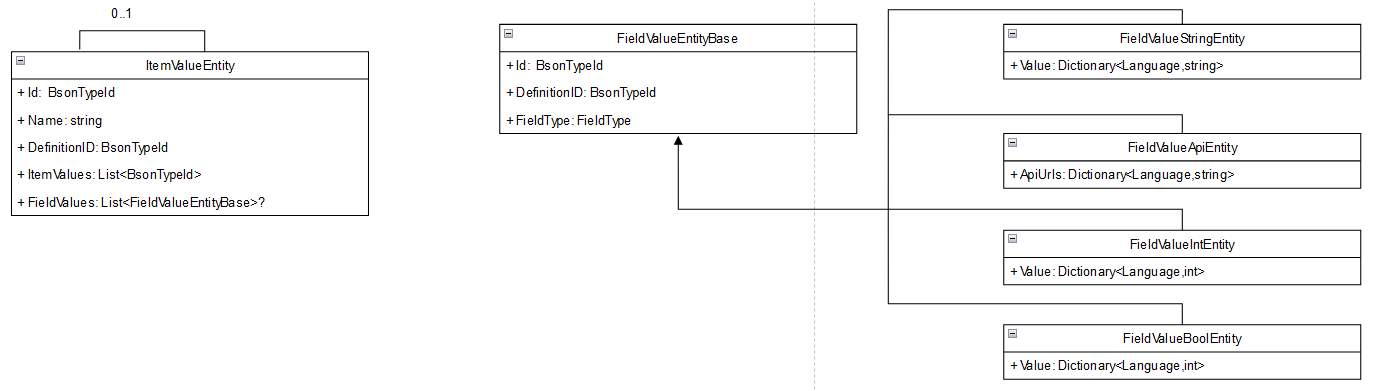
\includegraphics[scale=0.7]{ItemValueEntityClassDiagram.png}
    \label{fig:ItemValueEntityClassDiagram}
\end{graphic}

\whitespace[2]
\textbf{Item Definition}: Om structuur aan te geven aan de item values wordt er gebruik gemaakt van een item definition (zie figuur \ref{fig:ItemDefinitionClassDiagram}).
De belangrijkste functionaliteit van de definition is om aan te geven welke velden er op verschillende items zitten en welke daarvan verplicht zijn.

\whitespace[2]
\begin{graphic}
    \captionsetup{type=figure}
    \caption{Klassendiagram  ItemDefinition}
    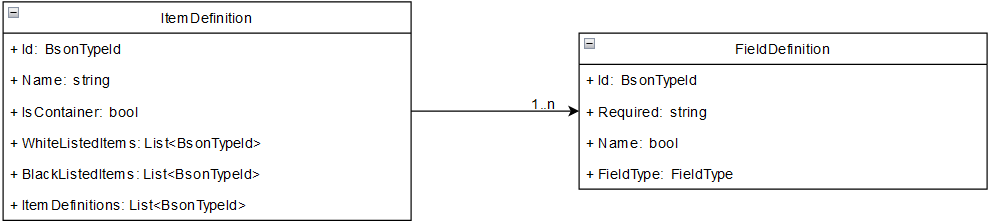
\includegraphics[scale=0.8]{ItemDefinitionClassDiagram.png}
    \label{fig:ItemDefinitionClassDiagram}
\end{graphic}

\whitespace
\textbf{VisualComponent}: Om de data te renderen moeten er components gebruikt worden in de frontend om dit af te handelen waar nodig.
De visualcomponent wordt gebruikt om deze componenten aan te geven welke er zijn en welke definition er bij hoordt.
Een klasse diagram van de visual component is te zien in figuur \ref{fig:VisualComponentEntityClassDiagram}.

\whitespace[2]
\begin{graphic}
    \captionsetup{type=figure}
    \caption{Klassendiagram VisualComponent}
    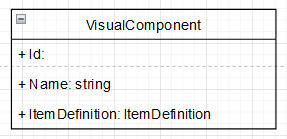
\includegraphics[scale=0.8]{VisualComponentEntityClassDiagram.png}
    \label{fig:VisualComponentEntityClassDiagram}
\end{graphic}

\whitespace[2]
\textbf{ItemVisual}: Dit is het object dat de visualcomponent en de item value samen voegt tot een geheel waardoor er content gerenderd kan worden op de pagina.
Verder geeft dit object ook aan welke mogelijke stijling of layout op het item moet worden toegepast (zie figuur \ref{fig:ItemVisualEntityClassDiagram}.
Om de data te renderen op een frontend wordt de itemVisual geparesed naar een itemvisualDTO zie figuur \ref{fig:ItemVisualDTOClassDiagram}.

\whitespace[2]
\begin{graphic}
	\captionsetup{type=figure}
	\caption{Klassendiagram ItemVisual}
	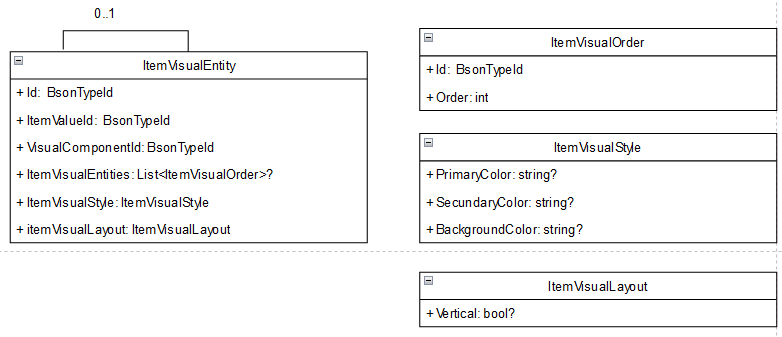
\includegraphics[scale=0.8]{ItemVisualEntityClassDiagram.png}
	\label{fig:ItemVisualEntityClassDiagram}
\end{graphic}

\whitespace[2]
\begin{graphic}
	\captionsetup{type=figure}
	\caption{Klassendiagram ItemVisualDTO}
	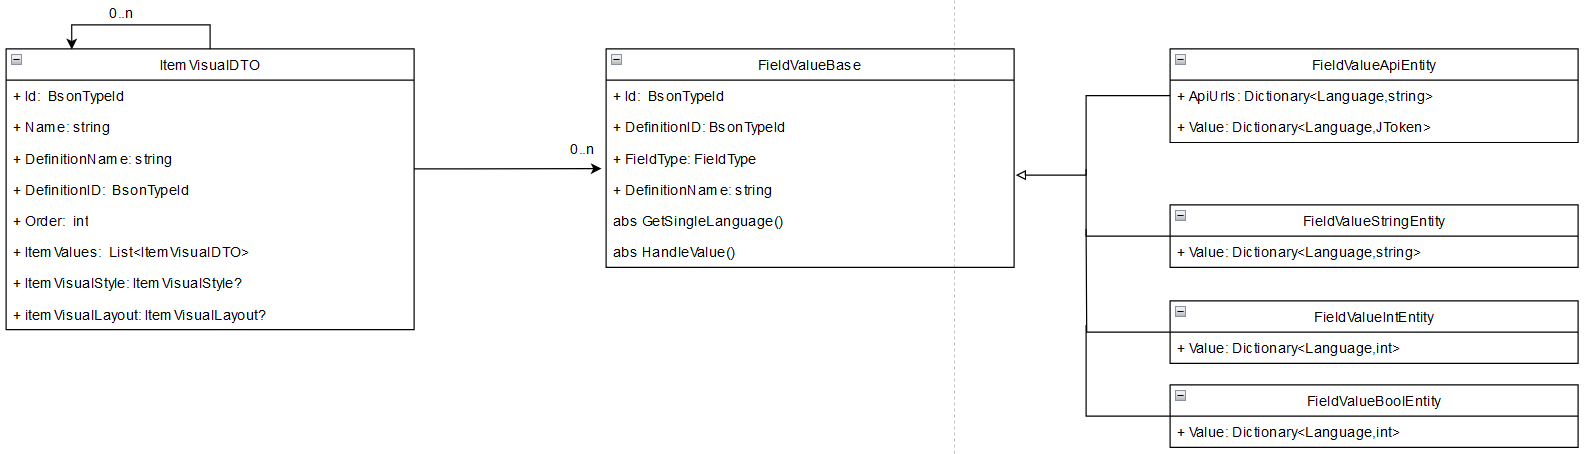
\includegraphics[scale=0.7]{ItemVisualDTO.png}
	\label{fig:ItemVisualDTOClassDiagram}
\end{graphic}
